\chapter{Periodograms}
\label{ch:axions-periodograms}
The space of possible axion--induced signals is spanned by their amplitude (the strength of the coupling) and their frequency (the axion mass). The problem is therefore naturally set in the frequency domain. We perform the analysis in two steps. First, we transform the measurements from the time domain into the frequency one by evaluating a \emph{periodogram} of it. The second step, the statistical treatment, is then easy.

In this section, we present the statistical methods we use. We start by defining the \emph{periodogram}, which serves as a transition from time to the frequency space, natural for looking for oscillations. Next we proceed to discuss the statistical properties of the periodogram, which lays the basis for this analysis.

For the sake of pedagogy we will discuss the methodology on a simple example.



\section{Definition}
A \emph{periodogram} is an estimator of the power spectrum. It has been proposed as the preferred way to treat periodic signals as early as 1898~\cite{Schuster1898}. In its simplest form it is the squared magnitude of the discrete Fourier transform. Lomb and Scargle have independently described a method one can construct a statistically well--behaving periodogram for non-uniformly sampled data with unequal error--bars: the Least Squares Spectral Analysis (LSSA)~\cite{Scargle1982}. It is also known as the Lomb--Scargle periodogram.

Many packages readily offer procedures to evaluate Lomb--Scargle periodograms~\cite{scipy,astropy}. They could not, however, be used directly as the analysis deviated in details from the standard procedure. We had to take a low--level approach, instead.

\begin{figure}
  \centering 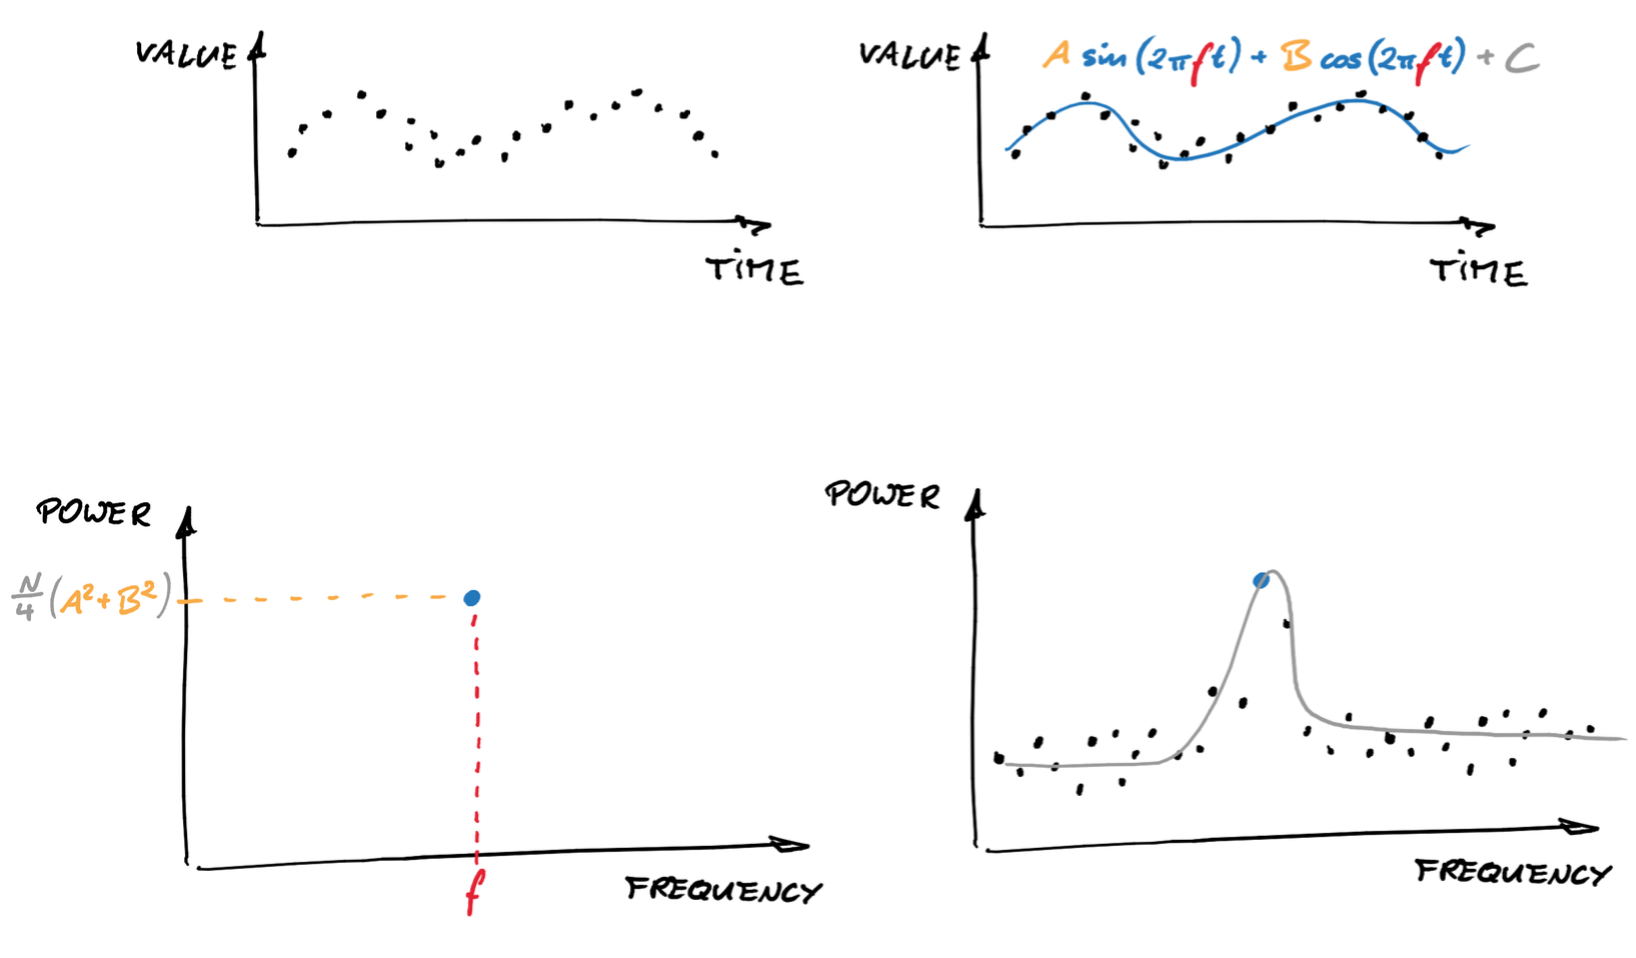
\includegraphics[width=\linewidth]{gfx/axions/LSSA}
  \caption{The LSSA periodogram, a function of frequency, is constructed by performing a linear least--squares fit at each of those frequencies.}
  \label{fig:LSSA_overview}
\end{figure}

To evaluate the LSSA periodogram at a circular frequency $\omega$, one performs a linear least--squares fit (hence the name) to the data with a function
\begin{equation}
  A\,\mathrm{cos}(\omega t) + B\,\mathrm{sin}(\omega t) + C \ ,
\end{equation}
where $A$, $B$ and $C$ are free parameters. The estimator of power $P(\omega)$ is then defined as
\begin{equation}
  P(\omega) := \frac{N}{4} \, \left( A^2 + B^2 \right) \ ,
\end{equation}
where $N$ is the number of data points. Different scaling factors may be used. We use the one of \cite{Scargle1982}, where the height of $\sqrt{P(\omega)}$ at the noise--bed corresponds numerically to the size of the error--bars squared, if they are all equal. LSSA, in contrast to the fast fourier transform (FFT), does not require windowing, because it is explicitly phase--aware. A graphical overview of the method is shown in Fig.\,\ref{fig:LSSA_overview}. Throughout the analysis, the figure of merit is either the power $P(\omega)$ or, interchangeably, its square root \emph{amplitude}. The latter has conveniently the same unit an the time series.

We will now follow an analysis of a simple example, shown in Fig.\,\ref{fig:basic_signal}. Despite being simple, is has already some properties of the actual dataset. The measurements are not equally spaced. They are grouped in 10--second long bunches, 20 seconds apart. Inside a bunch a measurement is taken every 2~seconds with a \unit[0.3]{s} jitter. The length of each measurement is 1~second with a \unit[0.1]{s} jitter. The error--bars are all size 1 in the arbitrary unit. An oscillating signal with an amplitude 0.7 and frequency \unit[0.17]{Hz}. Each measurement averages the signal over its duration.

\begin{figure}
  \centering 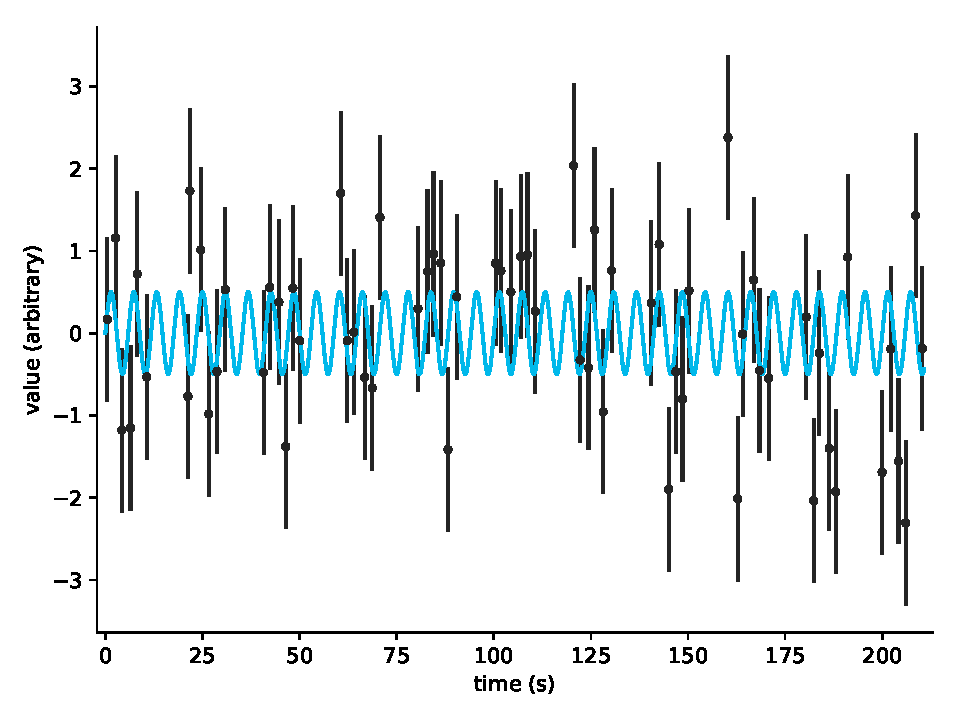
\includegraphics[width=0.8\linewidth]{gfx/axions/basic_signal.pdf}
  \caption{A simple signal generated just for the purpose for explaining the general scheme of periodogram analysis.}
  \label{fig:basic_signal}
\end{figure}

We proceed to evaluate the LSSA periodogram of this time series. The immediate question is: for which frequencies to evaluate the power? In case of equally--spaced series the upper limit is the \emph{Nyquist frequency}, equal to the half of the sampling rate~\cite{Shannon1949}. It is not the case when the sampling is not uniform. In practice we can expect little sensitivity to oscillations faster than the period over which each signal is averaged, \unit[1]{s} in the example. On the low side the limit is zero, which corresponds to the constant offset (an LSSA fit of a horizontal line, which is equivalent to calculating the average of the points).

When choosing the spacing between the frequencies we consider the the \emph{spectral resolution}, defined as the inverse span of the dataset. It roughly defines the minimal frequency difference between two signals that is distinguishable. In Fig.\,\ref{fig:basic_periodogram} there are two periodograms: evaluated at frequencies a spectral resolution apart (black dots), and one evaluated a thousand times more densely (the orange line). As no structure on a scale finer the the spectral resolution can be accessed, the orange line simply "connects" the black dots smoothly.

\begin{figure}
  \centering 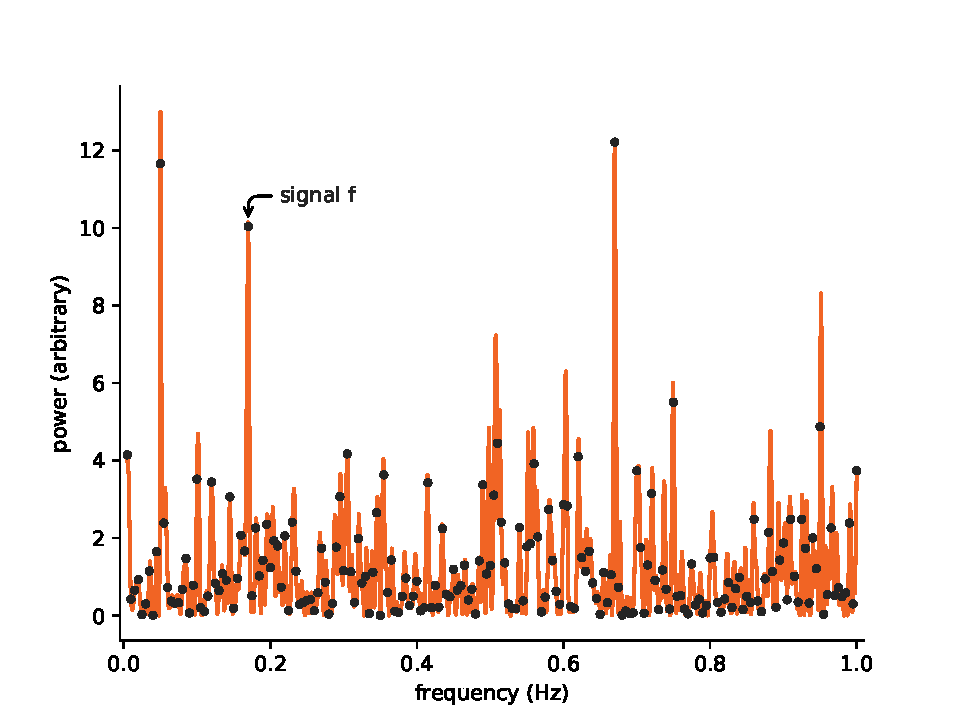
\includegraphics[width=0.8\linewidth]{gfx/axions/basic_periodogram.pdf}
  \caption{Two periodograms of the time series in Fig.\,\ref{fig:basic_signal}. One evaluated at frequencies a spectral resolution apart (black dots), and one evaluated a thousand times more densely (the orange line). As no structure on a scale finer the the spectral resolution can be accessed, the orange line simply "connects" the black dots.}
  \label{fig:basic_periodogram}
\end{figure}

In particular it is interesting to consider the difference between the 0 (offset) and the next frequency. Oscillations with a period longer than the span of the time series  appear in the series as a linear drift, if the measurements were taken in the linear part of the sine, or a quadratic change, if taken in the apex. Fitting such an oscillation is then equivalent to looking for a up--to--second--order drift in the data. Naturally, we expect the sensitivity to quickly worsen for these very long oscillations.

Fig.\,\ref{fig:basic_periodogram_loglog} shows the same two periodograms in a log--log scale. This scale is often used, as the potential signals span orders of magnitude in both frequency and amplitude. Unfortunately, it can lead to misunderstandings. Specifically, the noise appears to increase in amplitude with frequency. It is a purely cognitive effect. The spacing of the points is linear, so on a logarithmic scale the density of points increases for high amplitudes, making the extreme deviations more likely to appear in the same plot area, despite the noise amplitude being the same.

\begin{figure}
  \centering 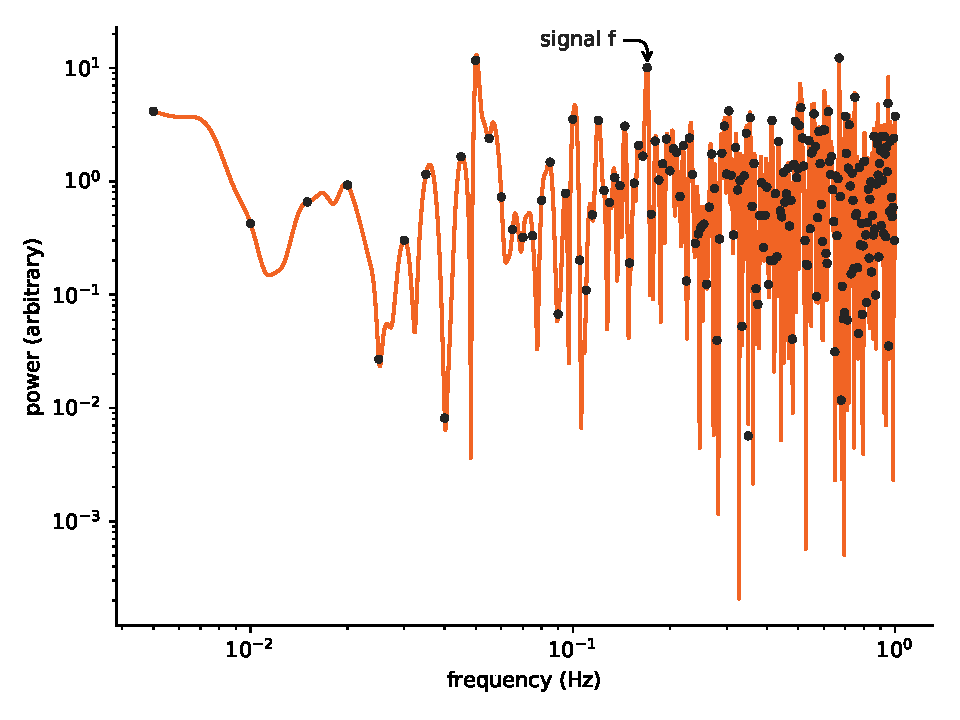
\includegraphics[width=0.8\linewidth]{gfx/axions/basic_periodogram_loglog.pdf}
  \caption{Two periodograms of the time series in Fig.\,\ref{fig:basic_signal}. One evaluated at frequencies a spectral resolution apart (black dots), and one evaluated a thousand times more densely (the orange line). As no structure on a scale finer the the spectral resolution can be accessed, the orange line simply "connects" the black dots. The periodogram is plotted on a log--log scale. The amplitude of the noise appears to be increasing with frequency, but it is not true. Only the density of the evaluated points increases, making the extreme deviations more pronounce.}
  \label{fig:basic_periodogram_loglog}
\end{figure}

An oscillation in the time series produces a peak in the periodogram. The position of the peak is the frequency of the oscillation, the width corresponds to the coherence of the signal. However, we see in the periodogram many peaks besides the one corresponding to the oscillation used when generating the data. Some are even bigger and there are many smaller ones. In the next section we will consider what, besides an oscillating signal, may give rise to a peak. Most importantly a way of determining whether a peak is caused by an oscillation is presented.




\section{A null hypothesis test}
\note{Mention that we roughly follow the reasoning of Scargle?}

Once the periodogram of a time series is calculated we would like to know whether it contains a signal signature. For a periodic signal this would be a peak. The really interesting statement is the answer to the question:

\begin{center}
  \emph{How likely is it that the highest peak in the periodogram is not only a random fluctuation?}
\end{center}

% We are, in fact, interested in the \emph{least likely} peak, which may not be the same as the highest one. For clarity we are going to be first considering the highest peak, and explain the difference later.

To describe the question mathematically, let us denote the time series of the real data by $D$. The peridogoram is then a set of $P^D(\omega_i)$, depicted with a black line in Fig.\,\ref{fig:basic_detection}. In a uniformly sampled case with equal error--bars we would expect $P^D(\omega_i)$ to be equally exponentially distributed for those frequencies where no signal is present ~\cite{Scargle1982}. In our, more complicated case, the distribution can be generated by a Monte Carlo (MC) simulation in the following way: a new signal is generated keeping the time position and the size of the error--bars, but with no underlying signal present -- the null hypothesis. The value for each simulated measurement is simply drawn from a gaussian distribution with the width corresponding to the size of the error--bar. Then the periodogram of the generated time series is calculated. This is repeated, yielding a set of periodograms, which are used to estimate the probability density function (PDF) of $P(\omega_i)$ for each $i$. The PDF for $\omega = \unit[0.17]{Hz}$ is depicted is the right--hand side of~Fig.\,\ref{fig:basic_detection}. In the left--hand side of this figure the 1-, 2- and $3\upsigma$ bands of the $P(\omega_i)$ PDFs are depicted in shades of green. For uniformly sampled data with equal error bars all PDFs would be the same and the $upsigma$ bands flat~\cite{Scargle1982}. In our case we see clear structures appearing, despite absolutely no signal being present in the generated time series.

\begin{figure}
  \centering 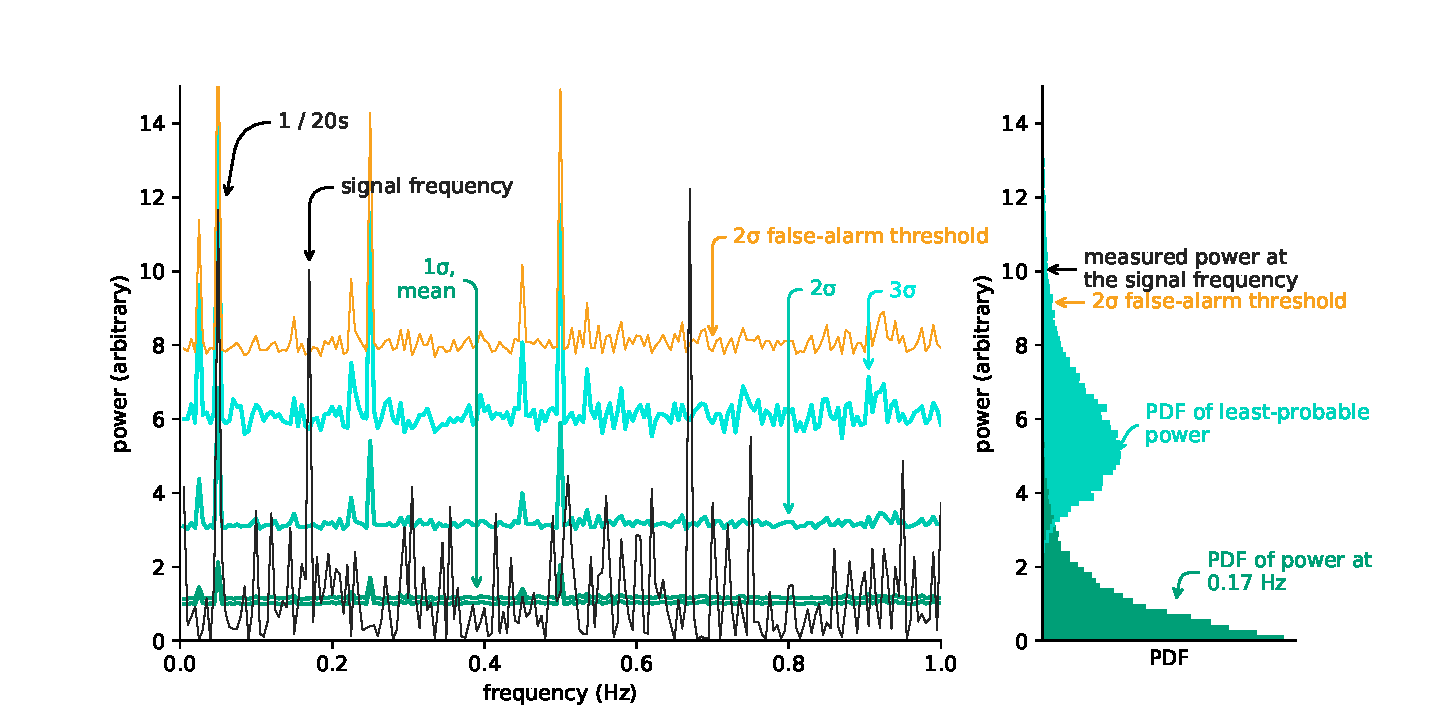
\includegraphics[width=\linewidth]{gfx/axions/basic_detection.pdf}
  \caption{A simple signal generated just for the purpose for explaining the general scheme of the analysis.}
  \label{fig:basic_detection}
\end{figure}

The structures in the $P(\omega_i)$ PDFs are caused solely by the nonuniformity in sampling times and in the sizes of the error--bars. In particular, we can identify a very large expected rise in power at \unit[0.05]{Hz}, corresponding exactly to the inverse spacing between the bunching (\unit[20]{s}) introduced in the example. Therefore, at this frequency we expect a peak to appear in the periodogram even when there is no significant oscillation of this frequency. This is the reason why we should consider the most significant peak, rather than simply the highest. This fact makes the presented reasoning different from the one of Scargle~\cite{Scargle1982}.

%We will be using the Cumulative Density Function (CDF) formalism.
We denote the cumulative density function (CDF) of the power estimator at the $i$-th frequency as $F_i(z)$ ($z$ would be the power estimated at frequency $\omega_i$). In an evenly sampled, no signal case it has a functional form:
\begin{equation}
  F_i(z) = 1 - e^{-z}
\end{equation}
In our case it can be estimated from the MC simulations. Then the $i$-th p-value is directly:
\begin{equation} \label{eq:local_p_value}
  p_i = 1 - F_i\left( P^D(\omega_i) \right)
\end{equation}
The most significant peak is the one with the lowest p-value. Yet, we can see that in the example signal there are 15 peaks with p-values on a 2$\upsigma$ level, much more than we would expect (a 2$\upsigma$ is a five--in--a--hundred event). This is due to the so--called \emph{look--elsewhere effect}, best explained as follows: a one--in--a--thousand event in a system is not a surprise, if it occurs in one of a thousand different systems. By looking at the Fig.\,\ref{fig:basic_detection} and comparing the periodogram of the signal with the $\upsigma$ bands, one essentially performs many, as many as the number of frequencies, largely independent statistical tests, cherry--picking among them the most significant peaks. The $p_i$ p-values are called \emph{local}, because they only measure the local significance at $\omega_i$.

There is an another way of understanding this phenomenon. The height of the most significant peak is a statistic itself. Its distribution can also be estimated from the MC--generated null hypothesis signals. The distribution is depicted on the right--hand size in Fig.\,\ref{fig:basic_detection} in \note{orange}. We can see that even when no signal is present, the highest peak will most of the times have a height placing it between 2- and 3$\upsigma$ local significance bands.

% The highest peak is then:
% \begin{align}
%   P_{max}^D &:= \mathrm{max}_i\,P^D(\omega_i) \\
%   \omega_{max}^D &:= \mathrm{arg\,max}_{\omega_i}\,P^D(\omega_i)
% \end{align}
% The height of the maximum, $P_{max}^D$, is a statistic itself. We refer to it as \emph{global}, in contrast with the \emph{local} set of statistics $P^D(\omega_i)$. We consider the distribution of $P_{max}^{H_0}$ given the null hypothesis $H_0$, where the time array is an array of normally distributed random variables, with widths equal to the corresponding error--bars. The probability that a peak at least as high as the one observed arises as a random fluctuation is:
% \begin{equation}
%   % \mathrm{Pr}\left( P_{max}^{H_0} > P_{max}^D\ |\, H_0 \right) \ .
%   \mathrm{Pr}\left( P_{max}^{H_0} > P_{max}^D \right) \ .
% \end{equation}
% This value is called the \emph{false alarm probability} (see eg. \cite{Pandola2004}). It can be numerically calculated with the Monte Carlo method by generating random data according to the null hypothesis (Fig.\,\ref{fig:generating_null_hypothesis_periodogram}) and counting the relative number of cases when $P_{max}^{H_0} > P_{max}^D$. To claim a discovery, the \emph{false alarm probability} has to be at most in the range of $2.87\,\cdot\,10^{-7}$ (so--called 5--sigma) \cite{PDG2014}.



% \begin{figure}
%   \centering
%   \subfloat
%   % [The not--yet--real data tested against hypothetical signals. Each pixel is one signal hypothesis. The white line connects points of 95\% C.L., surrounding an exclusion region. Note how deep into low amplitudes the line goes for couple of frequencies. See the text for the explanation.]
%   {%\label{fig:axions_exclusion}
%   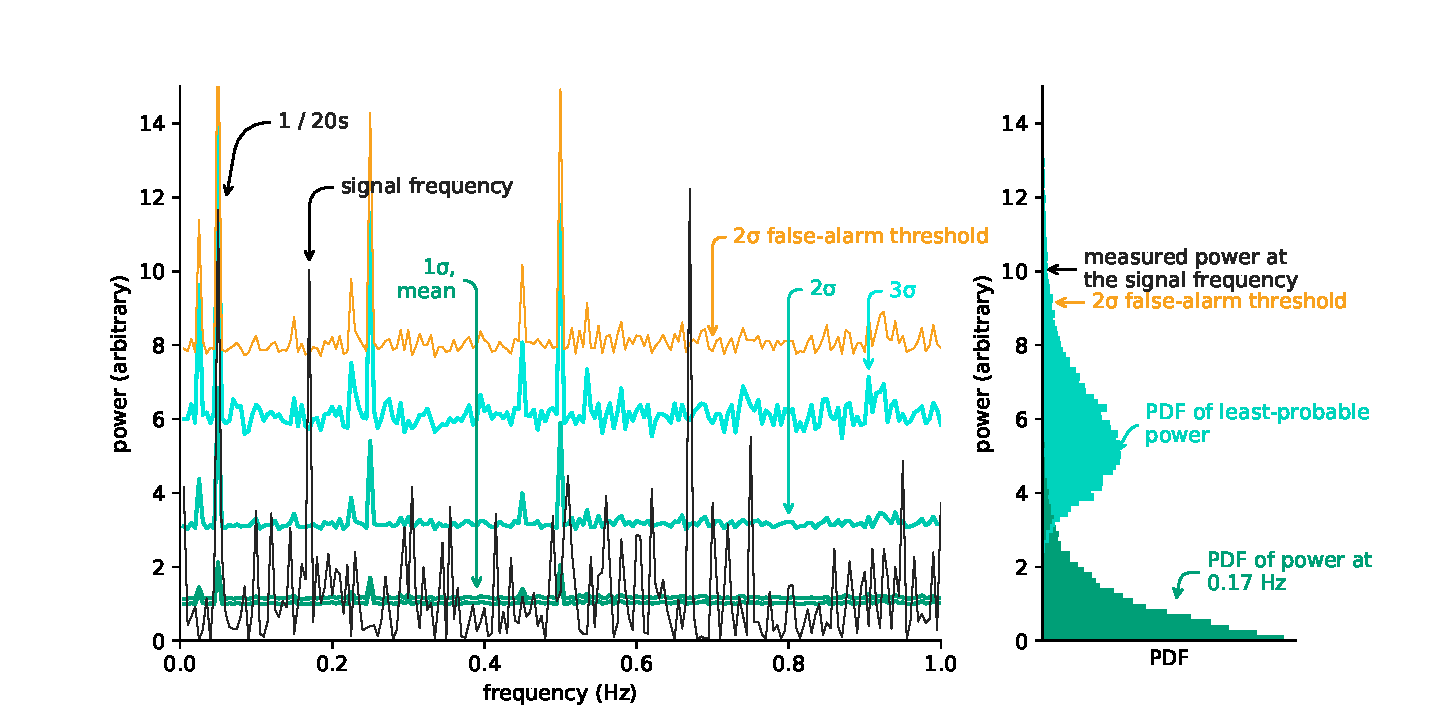
\includegraphics[width=.45\linewidth]{gfx/axions/basic_detection.pdf}}
%   \quad
%   \subfloat
%   % [The not--yet--real data tested against hypothetical signals using the \emph{CLs method}, in which hypotheses to which the experiment is not sensitive to get a statistical penalty. ]
%   {%\label{fig:basic_detection}
%   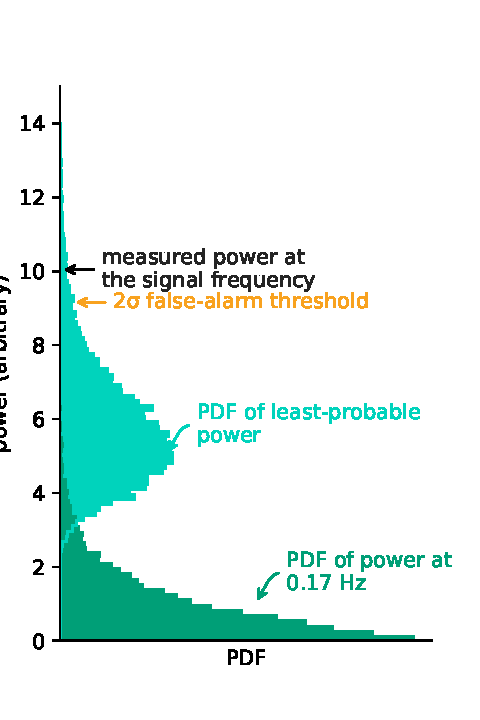
\includegraphics[width=.45\linewidth]{gfx/axions/basic_detection_histogram.pdf}}
%   \caption{Exclusion region --- signals that can be excluded at 95\% confidence level.}
%   \label{fig:basic_detection}
% \end{figure}

% It should be stressed that the distribution of $P_{max}$ is very different from the one of $P(\omega_{max})$. By looking for the highest peak, we check a big number of random variables $P(\omega_i)$ and pick a very special one --- the one that does lie the furthest in the tail of the distribution. The distribution of $P_{max}$ thus is centred around much higher values, as shown in Fig.\,\ref{fig:max_power_distribution}.

Let us now consider the local p--value of the most significant peak: $p_{\mathrm{min}} \, | H_0$. If the points of the periodogram were not correlated, this would be a simple case of many hypothesis testing \cite{Algeri2016}. The local p-values $p_i$ are, by definition, uniformly distributed. The CDF of a maximum of a set of uncorrelated variables is a product of their CDFs~\cite{Papoulis2002}. So in this case we have:
\begin{align}
  F_p(p) &= p \\
  F_{p_{max}}(p) &= p^N \\
  &\text{with}\ p' := 1 - p :\\
  F_{p_{min}}(p) &= 1 - F_{p'_{max}}(p') = 1 - (1 - p)^N \label{eq:Fpmin}\\
\end{align}
where $N$ is the number of frequencies tested. Correlations in the periodogram effectively lower $N$. If three dice are rolled in a way that two always give the same result, this is the same as rolling two dice when minimum roll is concerned. The CDF of $p_{\mathrm{min}} \, | H_0$, which we call $F^g$, can be estimated from the MC--generated data. Then the \emph{global} p-value is given by:
\begin{equation}
  p^g = F^g(p_{\mathrm{min}}^D)
\end{equation}

We can further determine \emph{false--alarm} thresholds. Traditionally, they are chosen to be at p-values of the normal distribution at $n \,\sigma$. The \emph{global} threshold p-value we call $p^g_{f.a.}$. The \emph{local} threshold p-value is:
\begin{equation}
  p_{f.a.} = \left( F^g \right)^{-1}(p^g_{f.a.})
\end{equation}
For each frequency the threshold power can be calculated:
\begin{equation}
  P^{f.a}_i = F_{P_i}^{-1}(1 - p_{f.a.})
\end{equation}
To claim a discovery, the \emph{false alarm probability} has to be at most in the range of $2.87\,\cdot\,10^{-7}$ (so--called 5--sigma) \cite{PDG2016}. The false--alarm thresholds for the example are depicted in Fig\,\ref{fig:basic_detection} in orange.

The amount of MC samples can be reduced, if the CDFs can be extrapolated. Effects like unequal error--bars and measurements of non--negligible duration causes them to deviate from the strictly derived equations in \cite{Scargle1982}. Nevertheless, we assume that functional form of the tails is preserved. Under the null hypothesis $F_{P_i}$ has form $1 - e^{-P}$ \cite{Scargle1982}. For $F^g$ we assume a form of Eq.\,(\ref{eq:Fpmin}), where $N$ is a parameter that we have to fit to account for correlations in the periodogram.

% In Fig.\,\ref{fig:ILL_detection} we present the periodogram of a fake ILL dataset (geneated with the same run timings and uncertainties as in the real dataset, with run EDM values generated according to gaussian distribution with mean of $0$ and standard deviation equal to that run's uncertainty). We decided not to analyse the real data set until we are fully happy with the method.
%
% \begin{figure}[h!]
%   \begin{center}
%     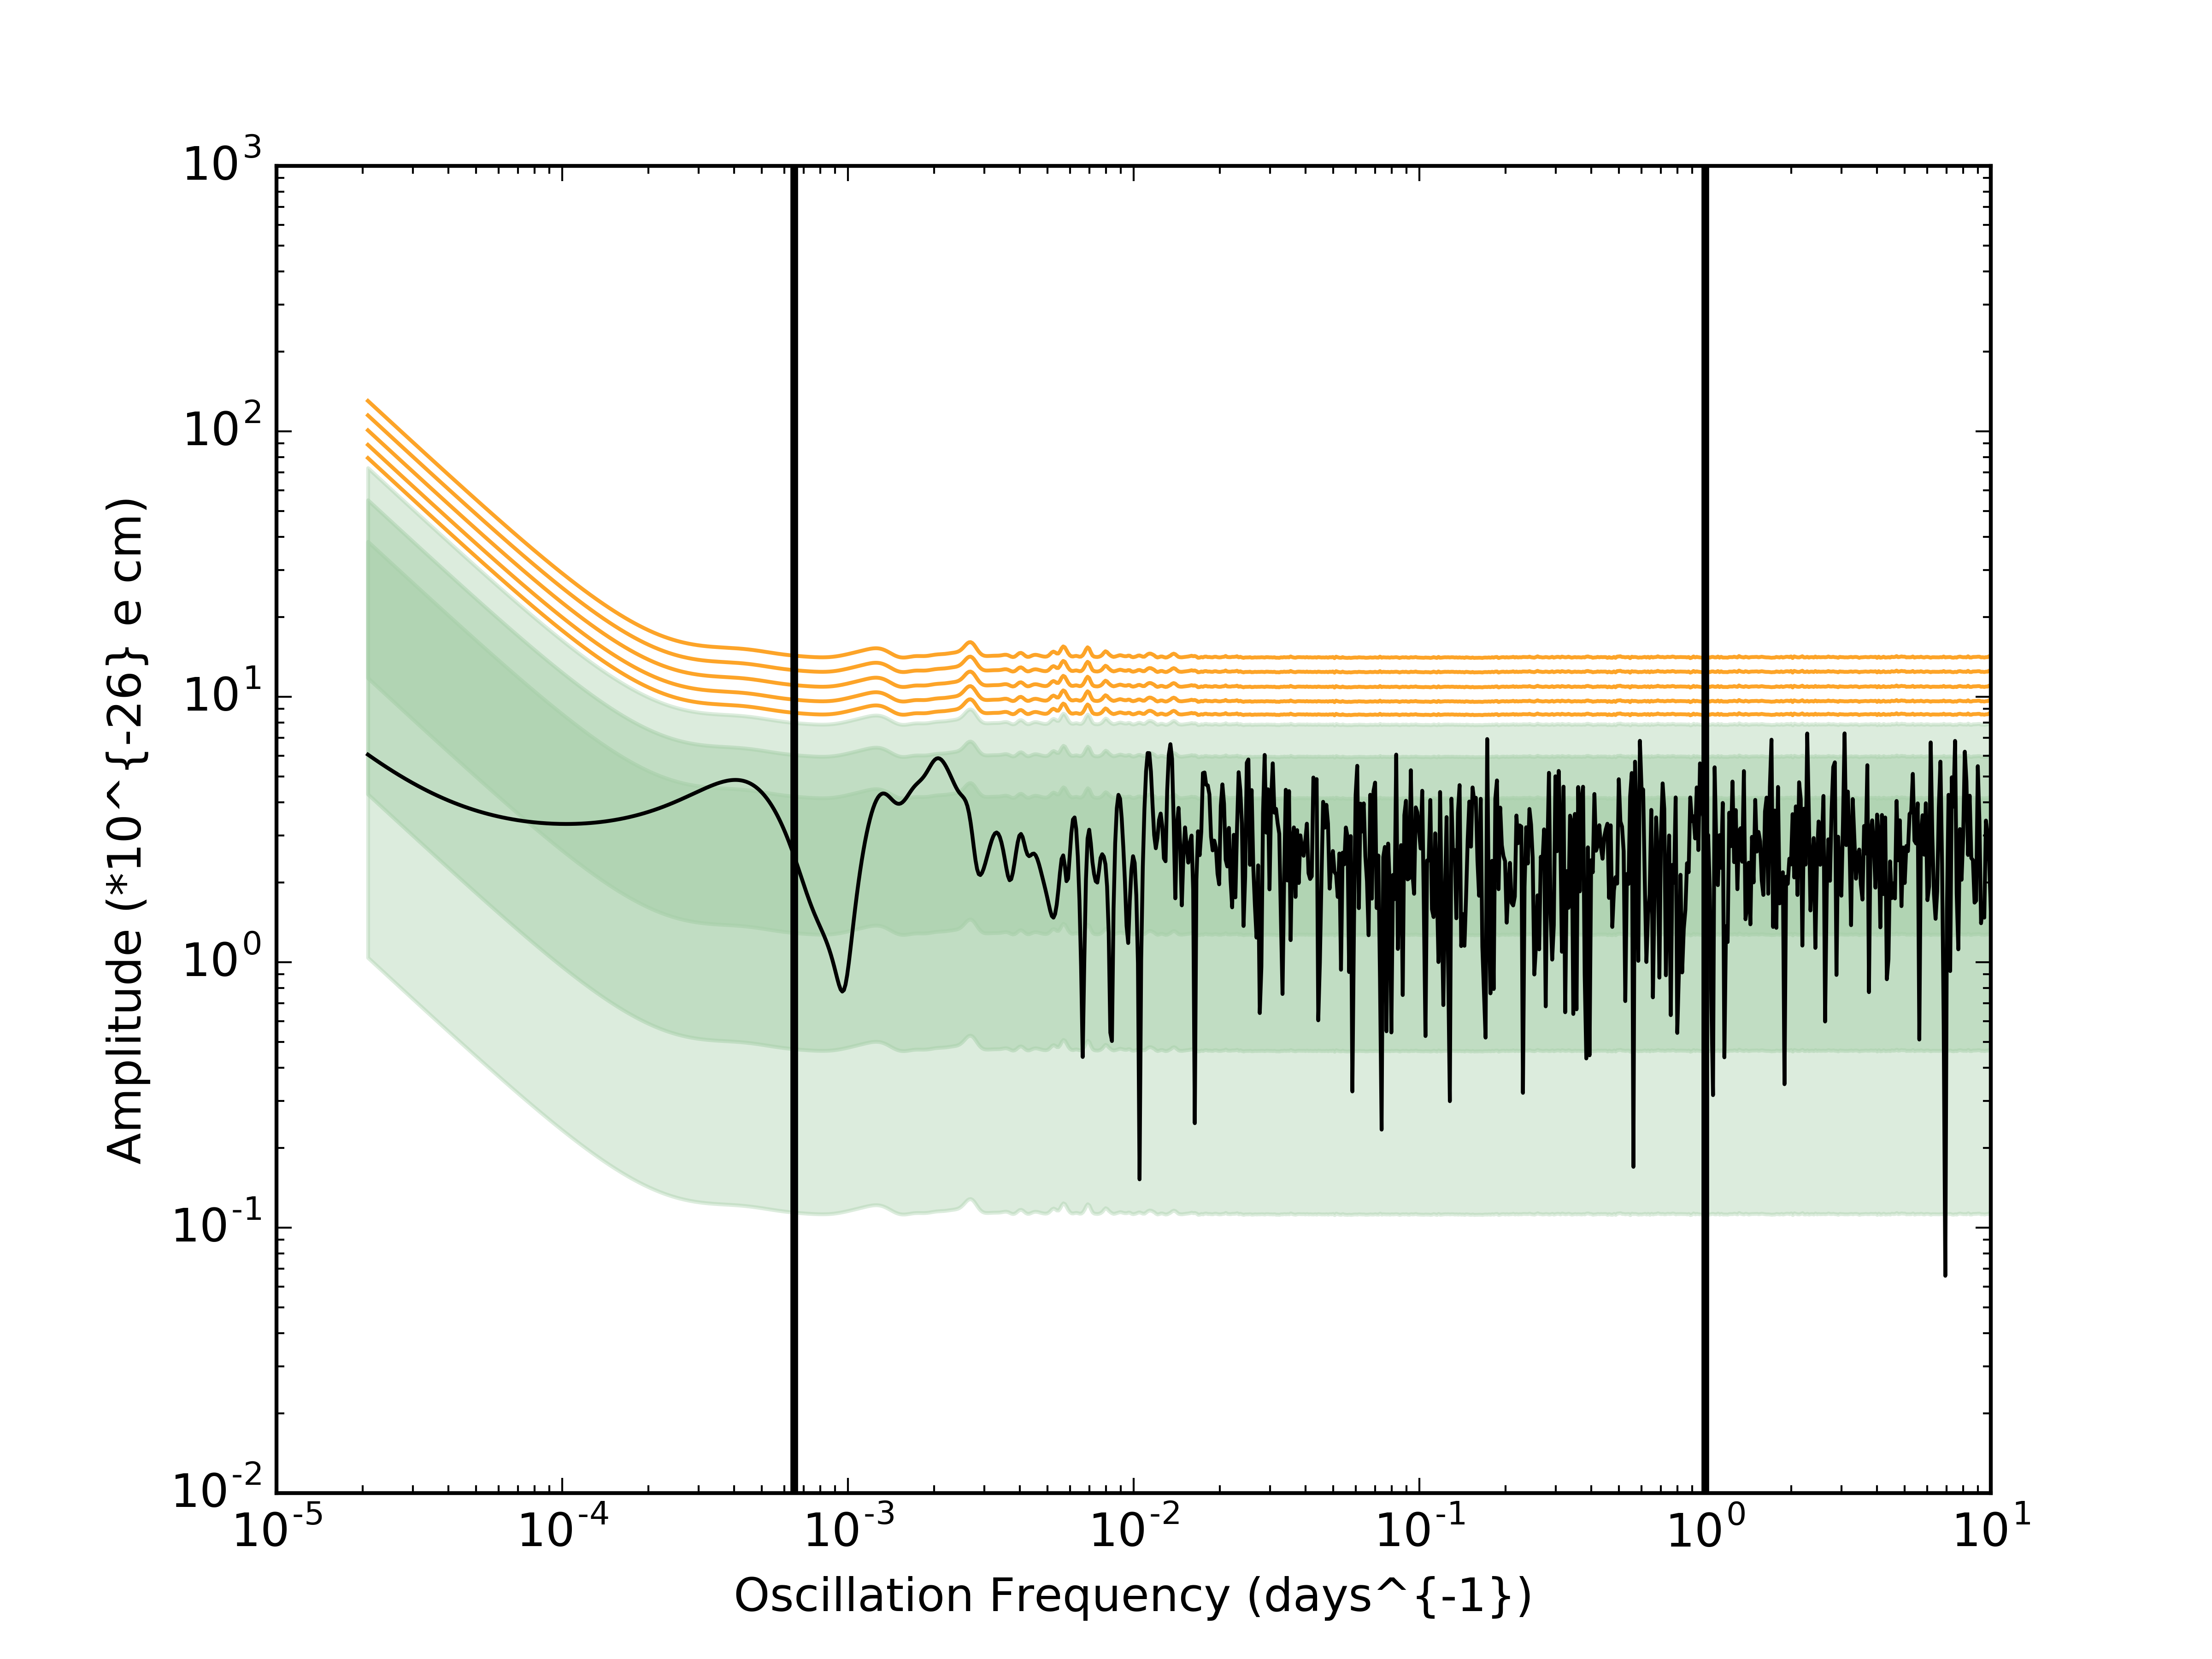
\includegraphics[width=\columnwidth]{gfx/axions/ILL_detection_Periodogram.png}
%     \caption{Periodogram of a fake ILL dataset. The green bands represent the distribution of the periodogram given the null hypothesis. The orange lines are 1-, 2-, 3-, 4-, 5--sigma false--alarm thresholds.}
%     \label{fig:ILL_detection}
%   \end{center}
% \end{figure}





\section{Signal hypotheses tests}
Should no claim for a discovery be possible, the next question to ask is:
\begin{center}
  \emph{Which oscillations would produce a visible peak, but did not, and can be thus excluded?}
\end{center}
In order to answer this question, the data need to be tested against being compatible with a number of model signal hypotheses. As an oscillation is characterised by its amplitude and frequency, the space of the hypotheses to test is two--dimensional.

\begin{figure}
  \centering 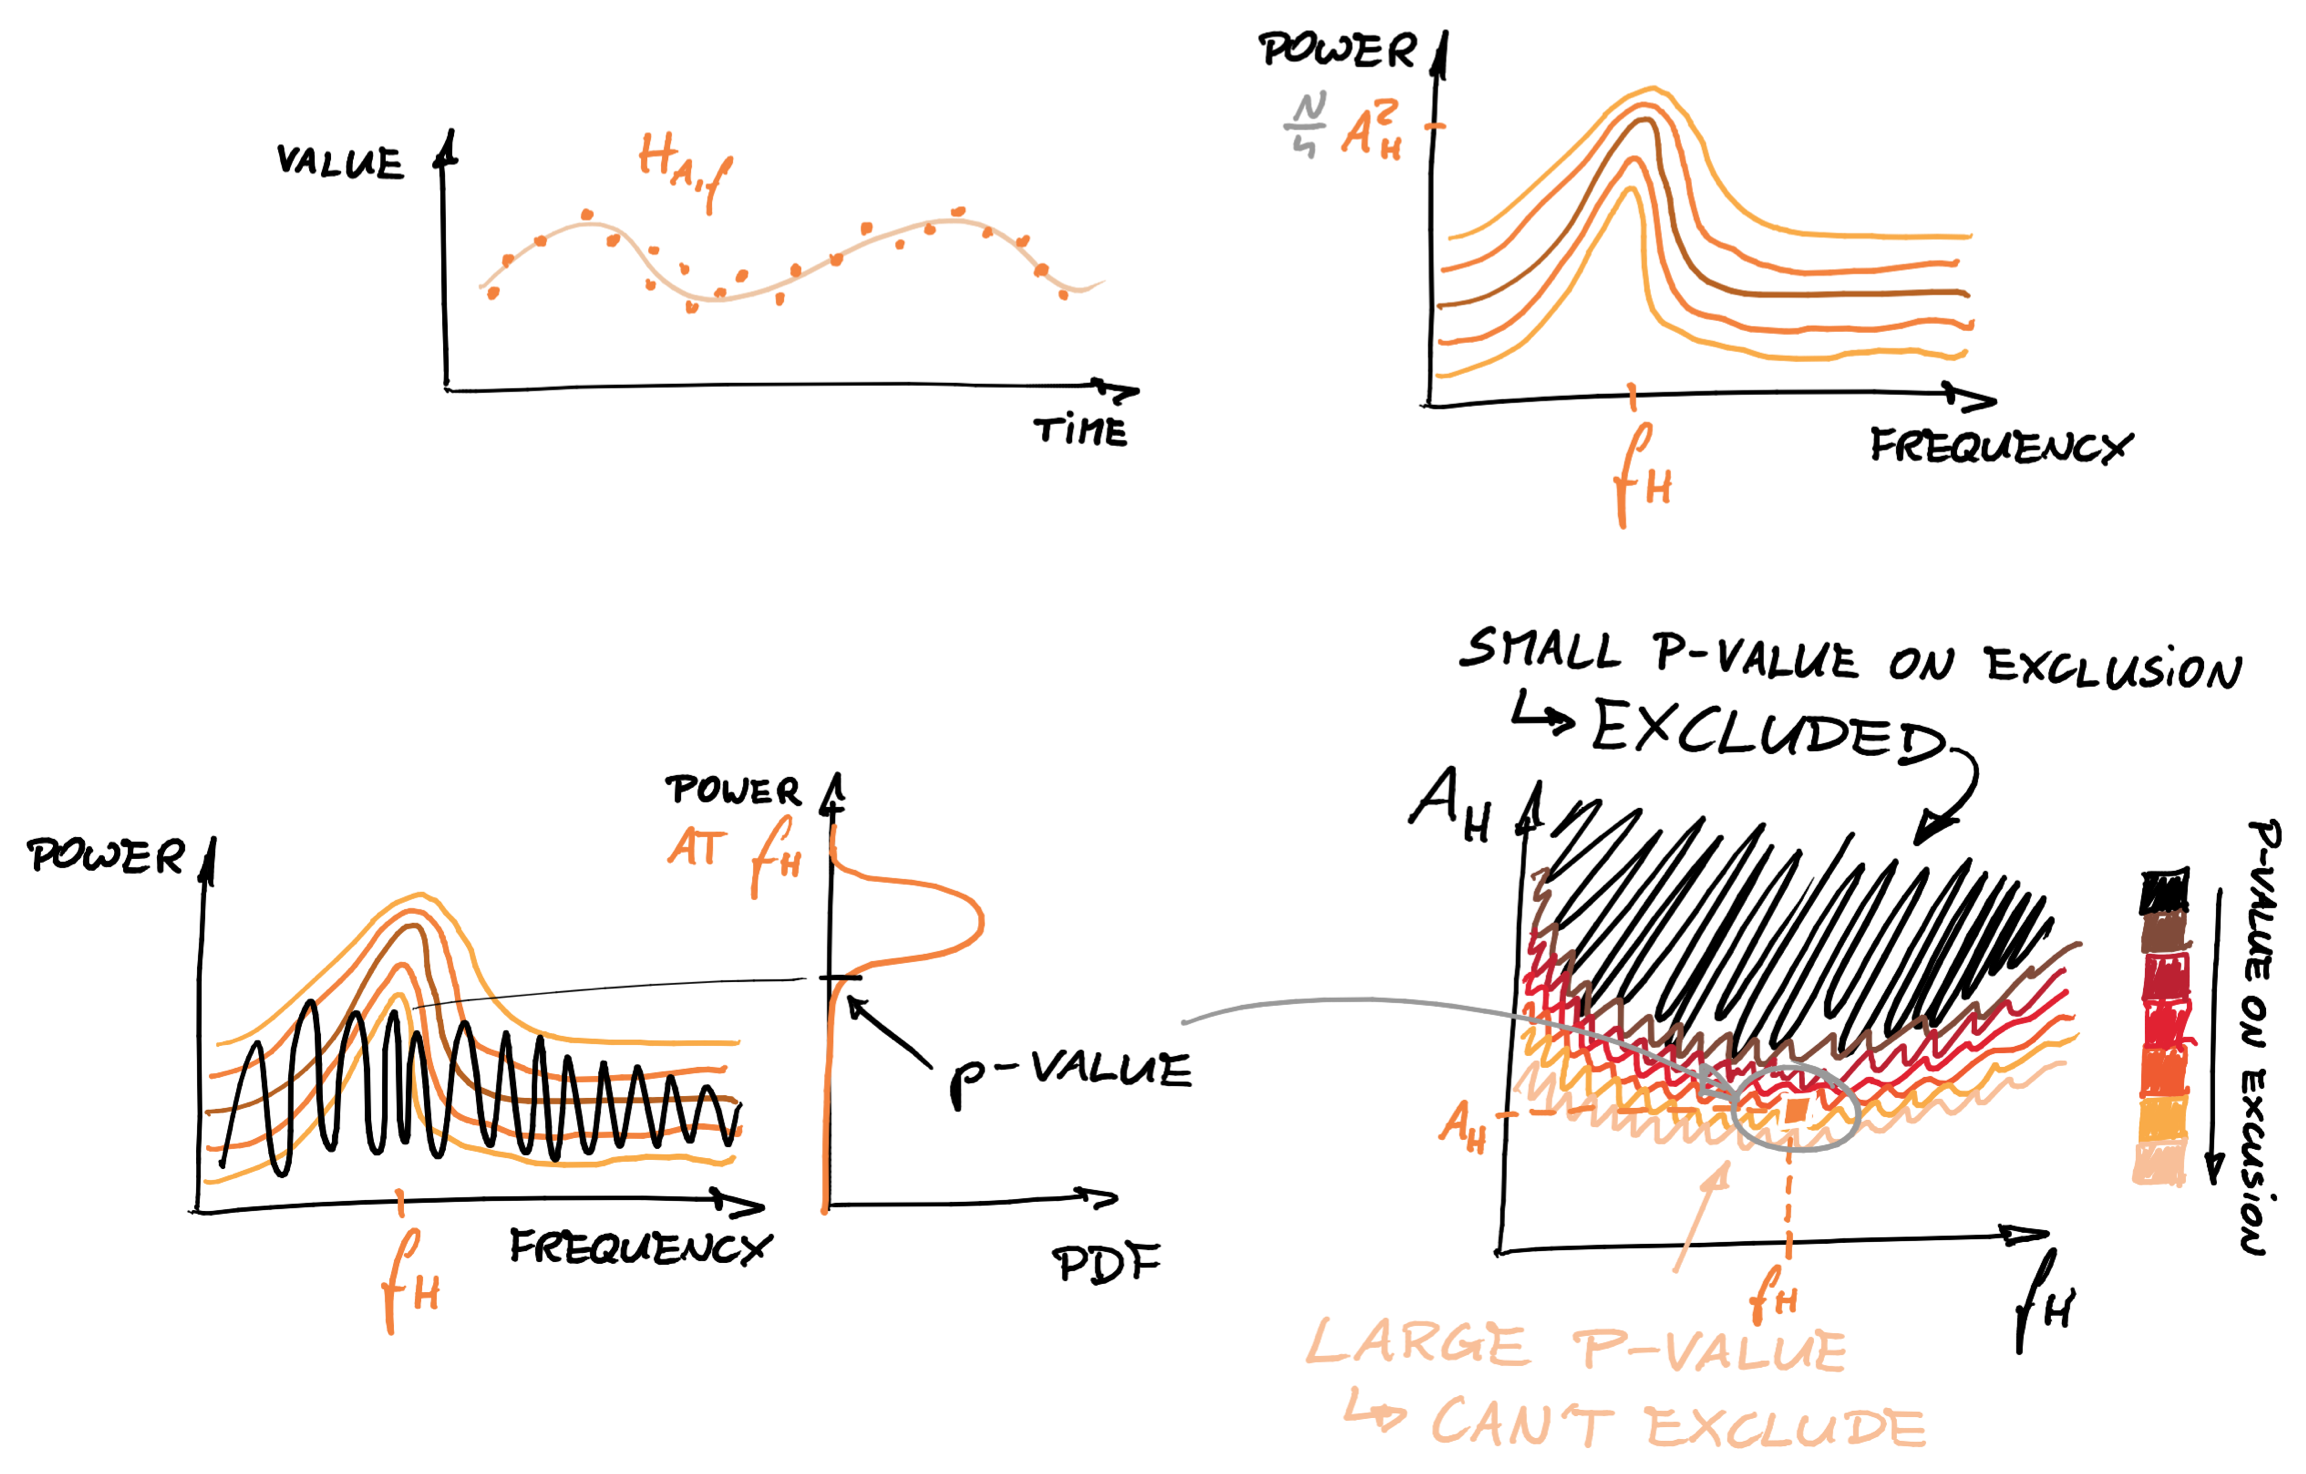
\includegraphics[width=\linewidth]{gfx/axions/exclusion_region.png}
  \caption{The general scheme of the exclusion limit determination. Note that in practice not the whole periodogram needs to be generated, but only its slice at $f_H$.}
  \label{fig:exclusion_region}
\end{figure}


\begin{figure}
  \centering 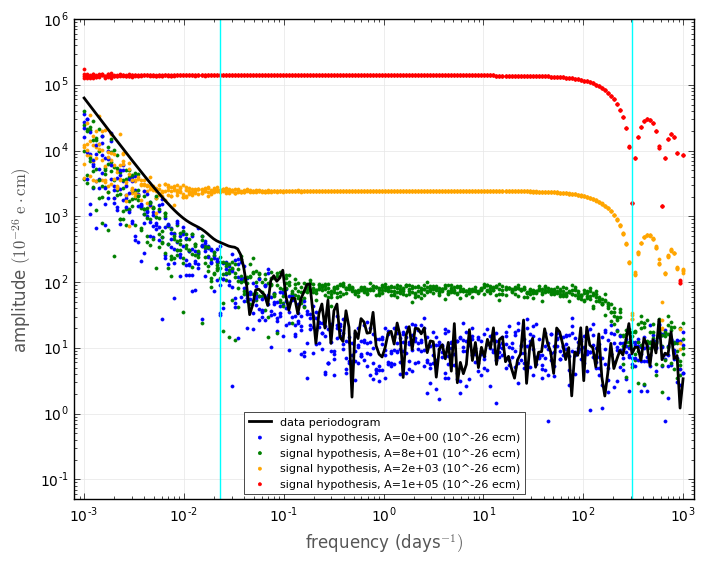
\includegraphics[width=\linewidth]{gfx/axions/sensitivity.png}
  \caption{For each frequency $f$, $\sqrt{\text{power}}$ is plotted for the dataset (black line) and MC--generated signal hypothesis of frequency $f$ and various amplitudes (different colours). For both high and low frequencies, the MC results approach the null hypothesis (blue). Also, a dip in power is nicely visible for oscillations coherent with the sampling frequency (and its multiples). The vertical lines depict the time--span of the dataset and the median separation between centres of runs.  The plot was produced with a test dataset, very different from the ILL dataset. \note{MR: It would be good for the sake of consistency to produce such a figure for the ILL fake dataset. - see fig \ref{fig:ILL_sensitivity}}}
  \label{fig:sensitivity}
\end{figure}


The probability that a hypothetical oscillation of amplitude $A$ and frequency $\omega$ would produce less power at frequency $\omega$ then observed is:
\begin{equation}
  % \mathrm{Pr}\left( P(\omega) < P^D(\omega)\ |\, H(\omega, A) \right) \ .
  \mathrm{Pr}\left( P^{H(\omega, A)}(\omega) < P^D(\omega)\ \right) \ .
\end{equation}
This probability is the p-value for the hypothesis $H(\omega, A)$ rejection. The distribution of $P^{H(\omega, A)}(\omega)$ is obtained with the Monte Carlo method. Here we also make use of CDF tail extrapolation \note{MR: This time, however, we extrapolate the low-power tail}, assuming a functional form as eq.\,(15) in \cite{Scargle1982} \note{MR: Not strictly, though. This equation behaves like linear function for very small $z$}. This test is repeated for different $\omega$ and $A$, each time covering a \emph{pixel} of the space of possible hypotheses. This procedure is shown schematically in Fig.\,\ref{fig:exclusion_region}. The set of hypotheses excluded at most at certain p-value forms an \emph{exclusion region}. We take the threshold p-value to be 5\%, which corresponds to a traditional confidence level of 95\%.

In this case, we cover the frequency spectrum much less densely than is the case in the null hypothesis test. This procedure is essentially evaluating the sensitivity of the measurement, which is solely determined by the timing and precision of the measurement points. We do not expect any highly resonant structures to appear therein.

During the Monte Carlo simulations we assume a perfectly coherent signal. The width of a real peak is not resolvable, as already mentioned.

% \begin{figure}
%   \myfloatalign
%   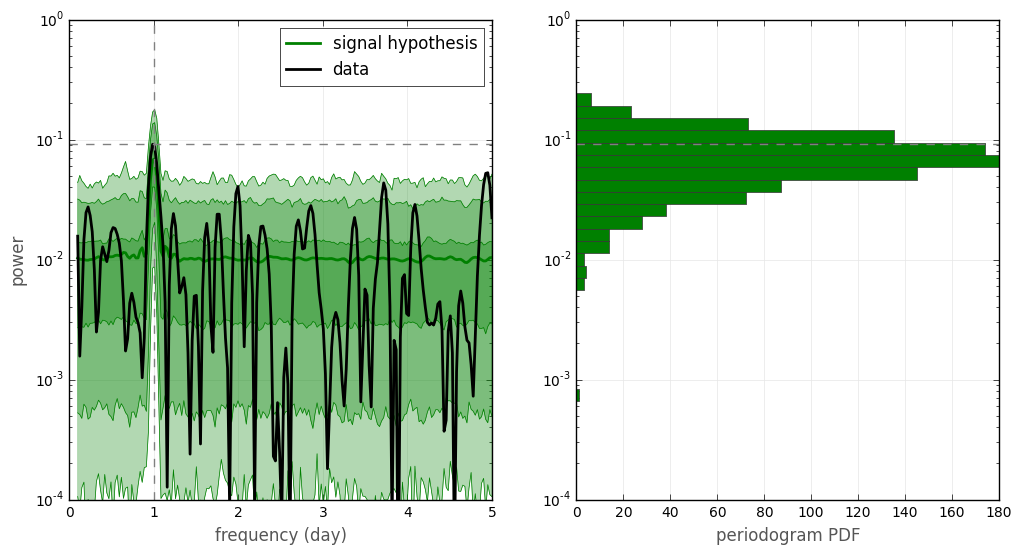
\includegraphics[width=.8\linewidth]{gfx/axions/axionMC_signal_hypothesis_rejection}
%   \caption
%   [...]
%   {
% \textsc{Left:} A periodogram of not--yet--real data on top of distribution of a periodogram of a hypothetical signal (green). \textsc{Right:} The distribution of power of the hypothetical signal at its model frequency.}
%   \label{fig:axions_signal_rejection}
% \end{figure}

\begin{figure}
  %FIXME directly copied from Elise's presentation on the 2015 PSI collaboration meeting
  \myfloatalign
  \subfloat
  [The not--yet--real data tested against hypothetical signals. Each pixel is one signal hypothesis. The white line connects points of 95\% C.L., surrounding an exclusion region. Note how deep into low amplitudes the line goes for couple of frequencies. See the text for the explanation.]
  {\label{fig:axions_exclusion_noCls}
  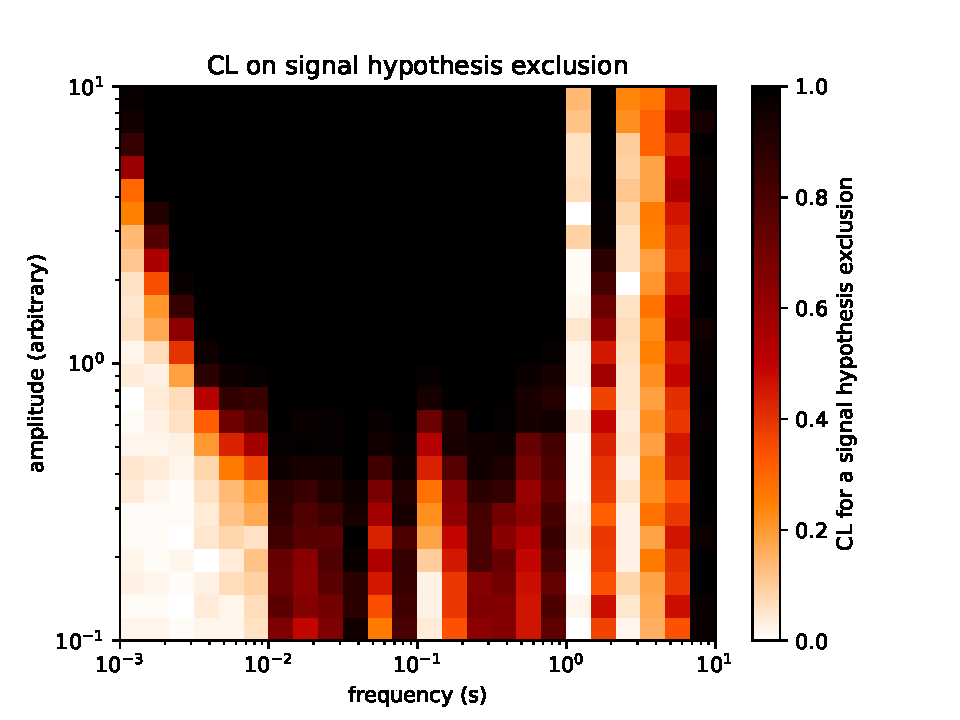
\includegraphics[width=.45\linewidth]{gfx/axions/basic_exclusion_noCls.pdf}}
  \quad
  \subfloat
  [The not--yet--real data tested against hypothetical signals using the \emph{CLs method}, in which hypotheses to which the experiment is not sensitive to get a statistical penalty. ]
  {\label{fig:axions_exclusion}
  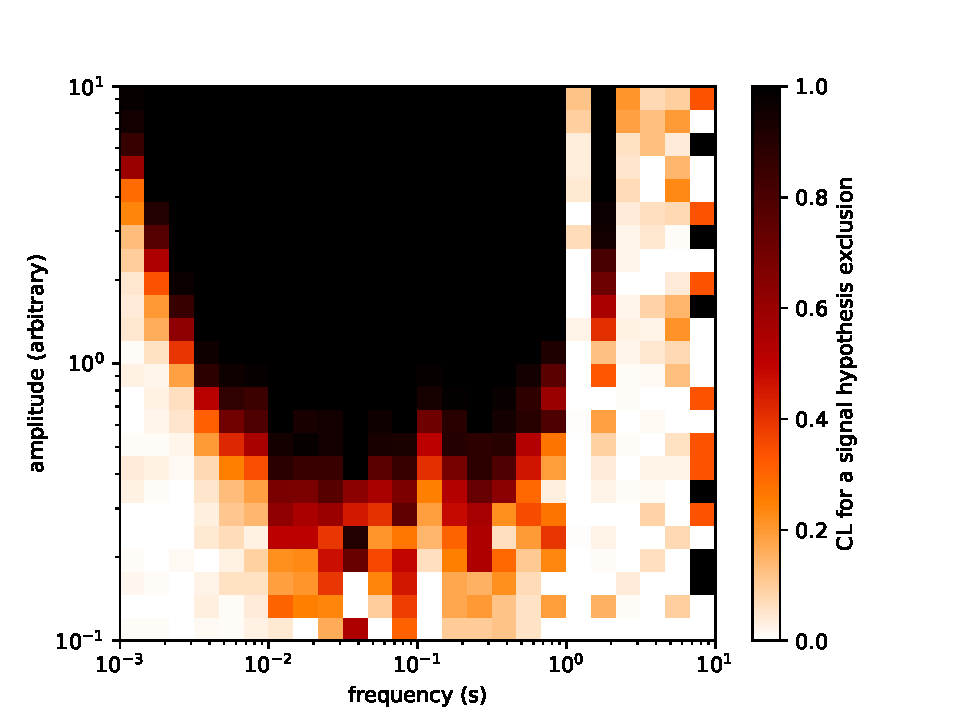
\includegraphics[width=.45\linewidth]{gfx/axions/basic_exclusion.pdf}}
  \caption{Exclusion region --- signals that can be excluded at 95\% confidence level..}
  \label{fig:axions_exclusions}
\end{figure}


The result of this procedure applied to a fake ILL dataset is presented on the left--hand side in Fig.\,\ref{fig:ILL_exclusion}. Looking at the exclusion region, one sees that the sensitivity to exclude drops for both high and low frequencies. This can be understood by looking at Fig.\,\ref{fig:sensitivity}, where the power obtained in the Monte Carlo generation for various hypotheses is plotted on top of the signal periodogram. For hypotheses with the same assumed amplitude of oscillation, the amplitude seen in the periodogram is constant for periods between the separation of the data points and the total length of the data set. Longer periods are harder to exclude, as it is always possible that one is near an antinode of an extremely slow oscillation. This manifests itself as a high amplitude seen even when the null hypothesis is assumed. High frequencies are suppressed because the experiment measures the average of the oscillation over a run. There little amplitude is visible, despite assuming an oscillation of a large amplitude. In particular there are dips at the approximate sampling frequency (the data have not been taken perfectly regularly) and its multiples.

\begin{figure}
  \centering 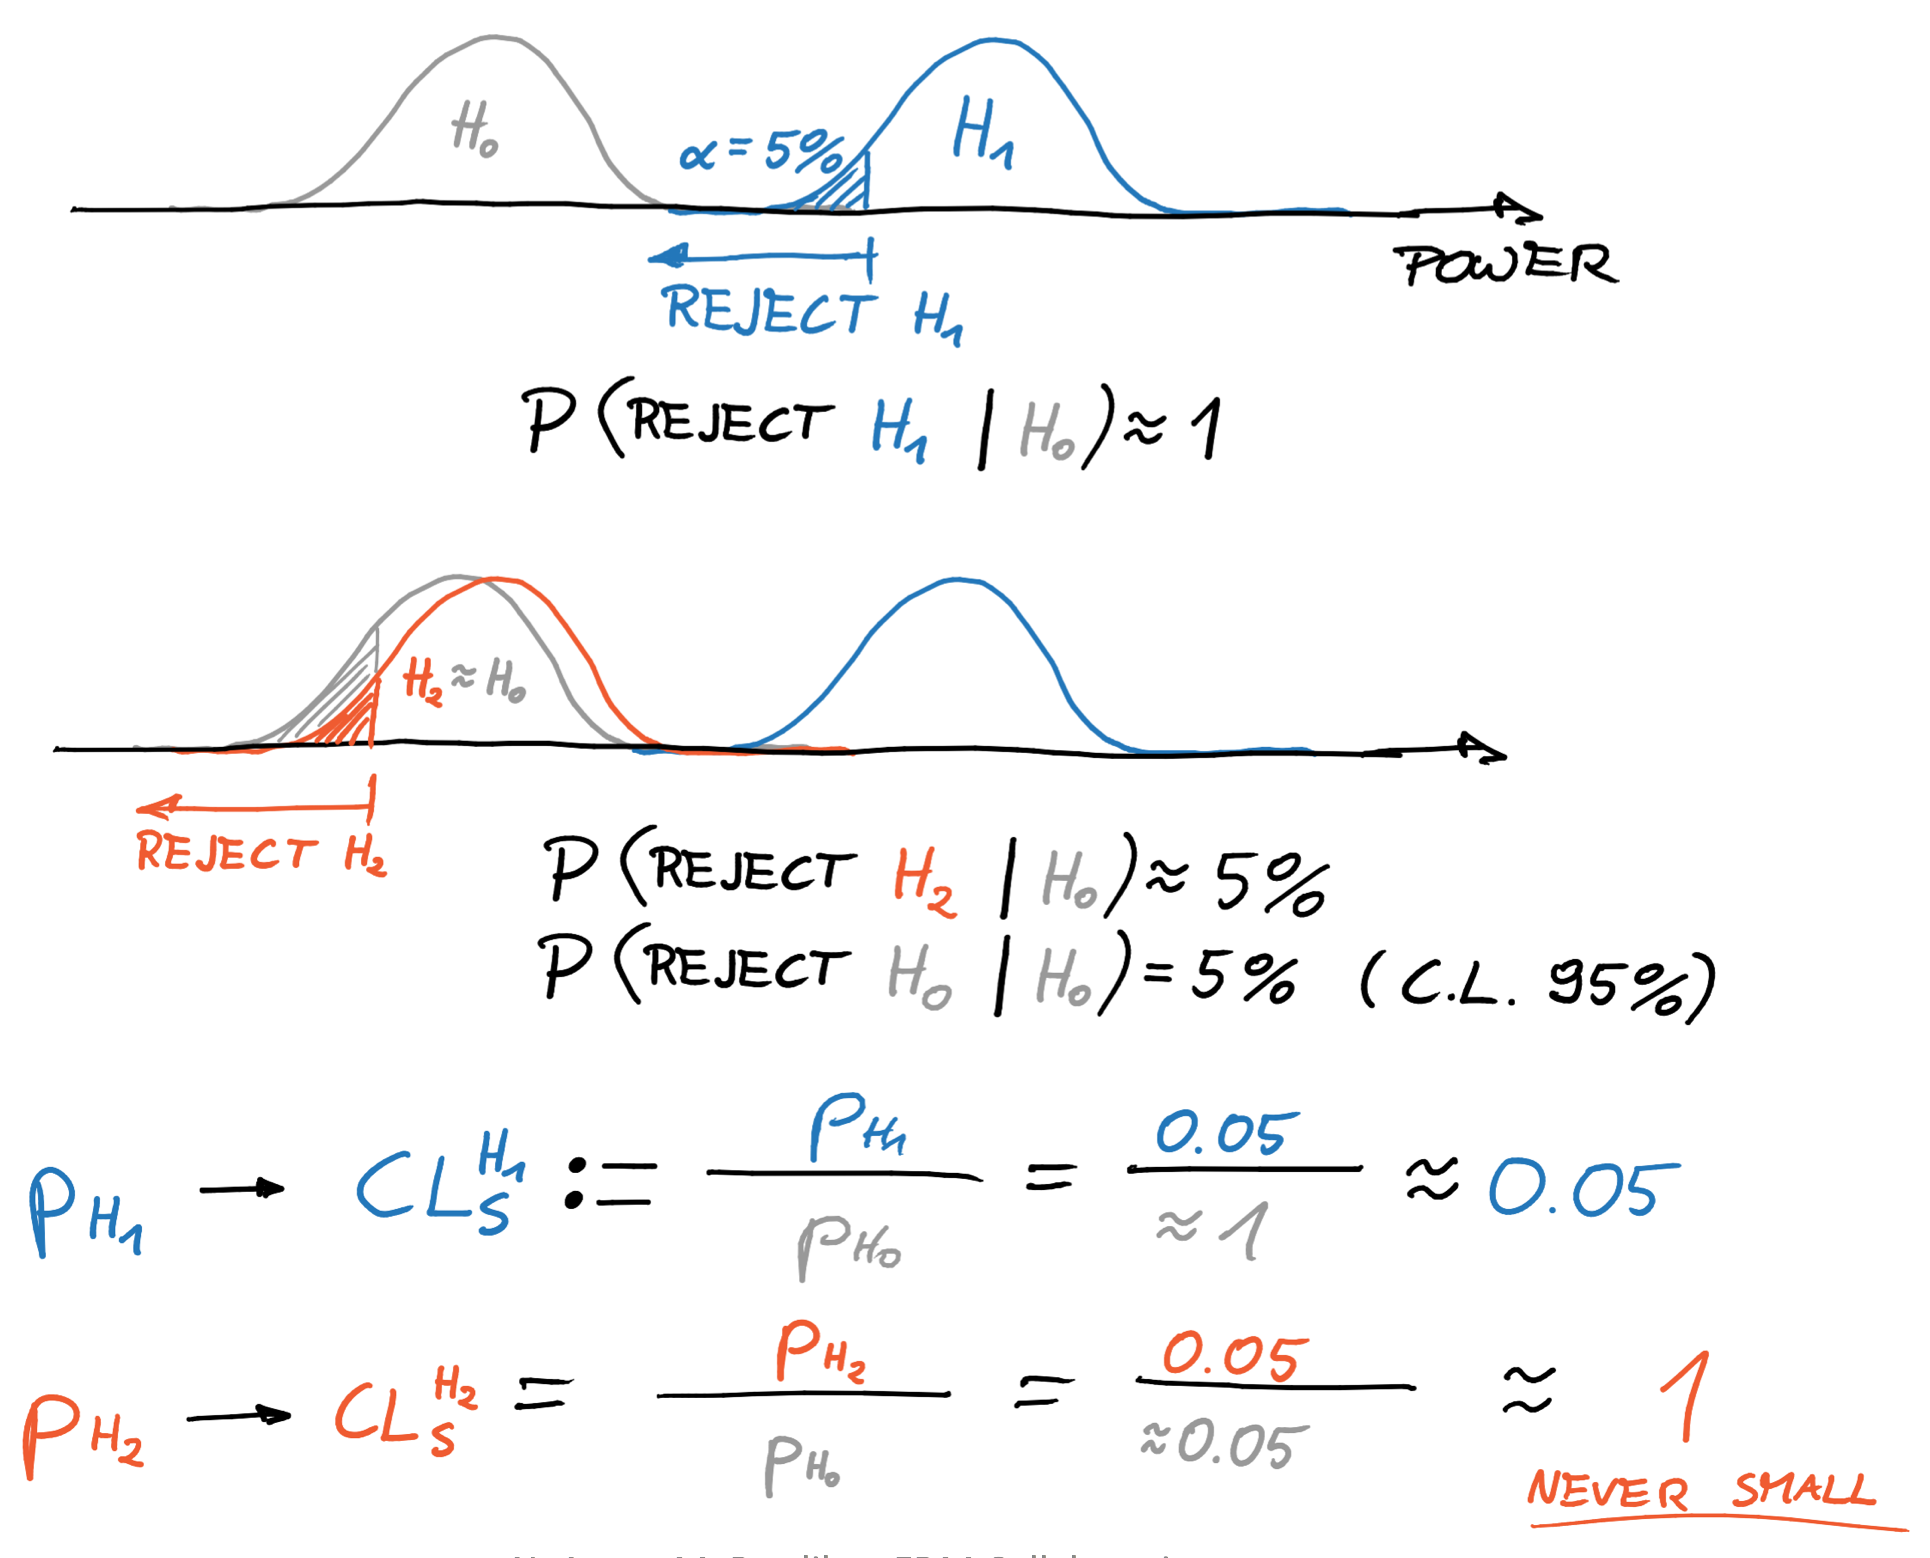
\includegraphics[width=\linewidth]{gfx/axions/CLs.png}
  \caption{The CLs method effectively suppresses power of hypotheses rejection if they are close to the null hypothesis.}
  \label{fig:CLs}
\end{figure}


The 95\%~C.L. exclusion region, depicted by a white line on the left--hand side in Fig.\,\ref{fig:exclusion_no_CLs}, exhibits a number of thin peaks going down in very low amplitudes. Seemingly, for some frequencies, signals with amplitude far below the sensitivity of the experiment are excluded. This is disturbing. Consider, however, that as the power was evaluated for many frequencies, inevitably at some of them, roughly 5\%, the power is low enough to be rejected at 95\%~C.L. even when tested against the null hypothesis. However completely fine from the statistical point of view, physicists do not accept a situation, where a hypothesis is rejected based on an experiment which was not sensitive to it. One possible solution is called the \emph{CLs method}. The method is defined, as well as the problem itself discussed, in the booklet of the Particle Data Group~\citep{PDG2014}. Here we only shortly present its idea graphically in Fig.\,\ref{fig:CLs}. With use of the \emph{CLs method} exclusion is suppressed in the region of low sensitivity, as shown on the right--hand side in Fig.\,\ref{fig:exclusion_no_CLs}.

Calculating each pixel of the alternative hypotheses space is largely a waste of resources. We are interested only in resolving the 95\% C.L. threshold. As a means of optimisation, we find the 95\% C.L. point for each frequency using the bisection algorithm. In only 10 steps it gives us relative precision below $0.01$ on its position. Thereby the final exclusion region is obtained \note{MR: figure needed, with the line only. It is missing for now for the run--level, but is present for the cycle--level}.
